% This file is generated by the MATLAB m-file laprint.m. It can be included
% into LaTeX documents using the packages graphicx, color and psfrag.
% It is accompanied by a postscript file. A sample LaTeX file is:
%    \documentclass{article}\usepackage{graphicx,color,psfrag}
%    \begin{document}% This file is generated by the MATLAB m-file laprint.m. It can be included
% into LaTeX documents using the packages graphicx, color and psfrag.
% It is accompanied by a postscript file. A sample LaTeX file is:
%    \documentclass{article}\usepackage{graphicx,color,psfrag}
%    \begin{document}% This file is generated by the MATLAB m-file laprint.m. It can be included
% into LaTeX documents using the packages graphicx, color and psfrag.
% It is accompanied by a postscript file. A sample LaTeX file is:
%    \documentclass{article}\usepackage{graphicx,color,psfrag}
%    \begin{document}% This file is generated by the MATLAB m-file laprint.m. It can be included
% into LaTeX documents using the packages graphicx, color and psfrag.
% It is accompanied by a postscript file. A sample LaTeX file is:
%    \documentclass{article}\usepackage{graphicx,color,psfrag}
%    \begin{document}\input{fig_4_6_tex}\end{document}
% See http://www.mathworks.de/matlabcentral/fileexchange/loadFile.do?objectId=4638
% for recent versions of laprint.m.
%
% created by:           LaPrint version 3.16 (13.9.2004)
% created on:           11-Jul-2009 20:16:30
% eps bounding box:     15 cm x 11.25 cm
% comment:              
%
\begin{psfrags}%
\psfragscanon%
%
% text strings:
\psfrag{s01}[lt][lt]{\color[rgb]{0,0,0}\setlength{\tabcolsep}{0pt}\begin{tabular}{l}x_1\end{tabular}}%
\psfrag{s02}[rt][rt]{\color[rgb]{0,0,0}\setlength{\tabcolsep}{0pt}\begin{tabular}{r}x_2\end{tabular}}%
\psfrag{s03}[b][b]{\color[rgb]{0,0,0}\setlength{\tabcolsep}{0pt}\begin{tabular}{c}x_3\end{tabular}}%
%
% xticklabels:
\psfrag{x01}[t][t]{-1}%
\psfrag{x02}[t][t]{-0.5}%
\psfrag{x03}[t][t]{0}%
\psfrag{x04}[t][t]{0.5}%
\psfrag{x05}[t][t]{1}%
\psfrag{x06}[t][t]{1.5}%
%
% yticklabels:
\psfrag{v01}[r][r]{-2}%
\psfrag{v02}[r][r]{-1}%
\psfrag{v03}[r][r]{0}%
\psfrag{v04}[r][r]{1}%
%
% zticklabels:
\psfrag{z01}[r][r]{0}%
\psfrag{z02}[r][r]{1}%
\psfrag{z03}[r][r]{2}%
\psfrag{z04}[r][r]{3}%
\psfrag{z05}[r][r]{4}%
\psfrag{z06}[r][r]{5}%
%
% Figure:
\resizebox{12cm}{!}{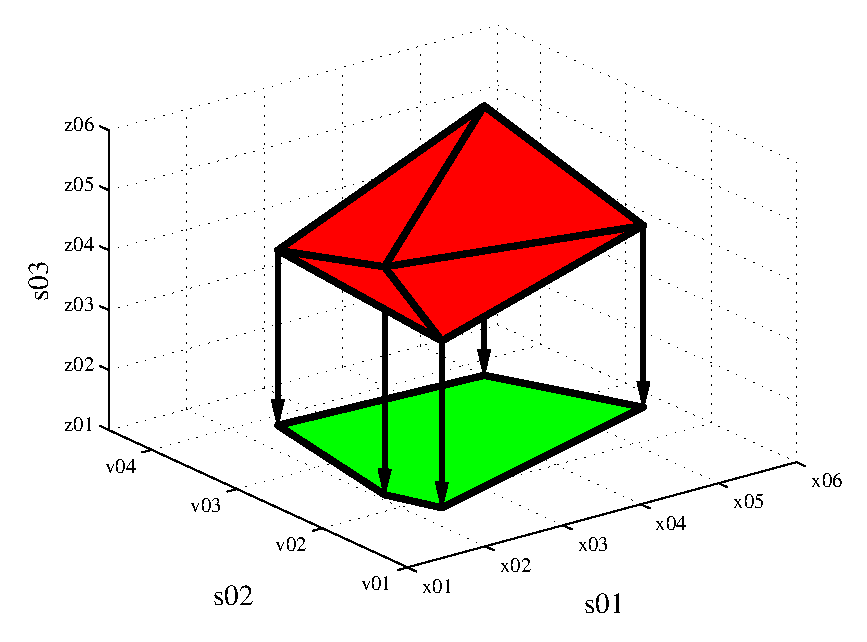
\includegraphics{fig_4_6_tex.eps}}%
\end{psfrags}%
%
% End fig_4_6_tex.tex
\end{document}
% See http://www.mathworks.de/matlabcentral/fileexchange/loadFile.do?objectId=4638
% for recent versions of laprint.m.
%
% created by:           LaPrint version 3.16 (13.9.2004)
% created on:           11-Jul-2009 20:16:30
% eps bounding box:     15 cm x 11.25 cm
% comment:              
%
\begin{psfrags}%
\psfragscanon%
%
% text strings:
\psfrag{s01}[lt][lt]{\color[rgb]{0,0,0}\setlength{\tabcolsep}{0pt}\begin{tabular}{l}x_1\end{tabular}}%
\psfrag{s02}[rt][rt]{\color[rgb]{0,0,0}\setlength{\tabcolsep}{0pt}\begin{tabular}{r}x_2\end{tabular}}%
\psfrag{s03}[b][b]{\color[rgb]{0,0,0}\setlength{\tabcolsep}{0pt}\begin{tabular}{c}x_3\end{tabular}}%
%
% xticklabels:
\psfrag{x01}[t][t]{-1}%
\psfrag{x02}[t][t]{-0.5}%
\psfrag{x03}[t][t]{0}%
\psfrag{x04}[t][t]{0.5}%
\psfrag{x05}[t][t]{1}%
\psfrag{x06}[t][t]{1.5}%
%
% yticklabels:
\psfrag{v01}[r][r]{-2}%
\psfrag{v02}[r][r]{-1}%
\psfrag{v03}[r][r]{0}%
\psfrag{v04}[r][r]{1}%
%
% zticklabels:
\psfrag{z01}[r][r]{0}%
\psfrag{z02}[r][r]{1}%
\psfrag{z03}[r][r]{2}%
\psfrag{z04}[r][r]{3}%
\psfrag{z05}[r][r]{4}%
\psfrag{z06}[r][r]{5}%
%
% Figure:
\resizebox{12cm}{!}{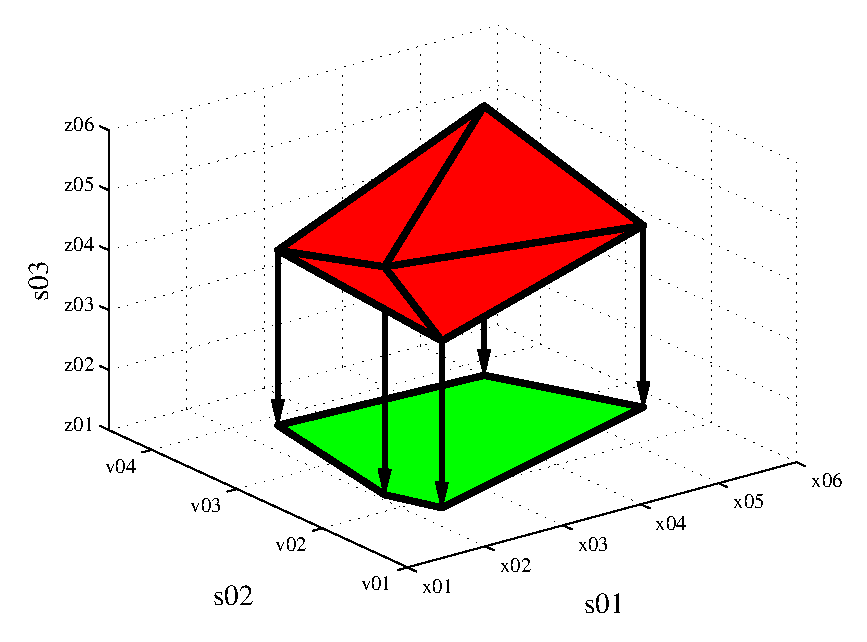
\includegraphics{fig_4_6_tex.eps}}%
\end{psfrags}%
%
% End fig_4_6_tex.tex
\end{document}
% See http://www.mathworks.de/matlabcentral/fileexchange/loadFile.do?objectId=4638
% for recent versions of laprint.m.
%
% created by:           LaPrint version 3.16 (13.9.2004)
% created on:           11-Jul-2009 20:16:30
% eps bounding box:     15 cm x 11.25 cm
% comment:              
%
\begin{psfrags}%
\psfragscanon%
%
% text strings:
\psfrag{s01}[lt][lt]{\color[rgb]{0,0,0}\setlength{\tabcolsep}{0pt}\begin{tabular}{l}x_1\end{tabular}}%
\psfrag{s02}[rt][rt]{\color[rgb]{0,0,0}\setlength{\tabcolsep}{0pt}\begin{tabular}{r}x_2\end{tabular}}%
\psfrag{s03}[b][b]{\color[rgb]{0,0,0}\setlength{\tabcolsep}{0pt}\begin{tabular}{c}x_3\end{tabular}}%
%
% xticklabels:
\psfrag{x01}[t][t]{-1}%
\psfrag{x02}[t][t]{-0.5}%
\psfrag{x03}[t][t]{0}%
\psfrag{x04}[t][t]{0.5}%
\psfrag{x05}[t][t]{1}%
\psfrag{x06}[t][t]{1.5}%
%
% yticklabels:
\psfrag{v01}[r][r]{-2}%
\psfrag{v02}[r][r]{-1}%
\psfrag{v03}[r][r]{0}%
\psfrag{v04}[r][r]{1}%
%
% zticklabels:
\psfrag{z01}[r][r]{0}%
\psfrag{z02}[r][r]{1}%
\psfrag{z03}[r][r]{2}%
\psfrag{z04}[r][r]{3}%
\psfrag{z05}[r][r]{4}%
\psfrag{z06}[r][r]{5}%
%
% Figure:
\resizebox{12cm}{!}{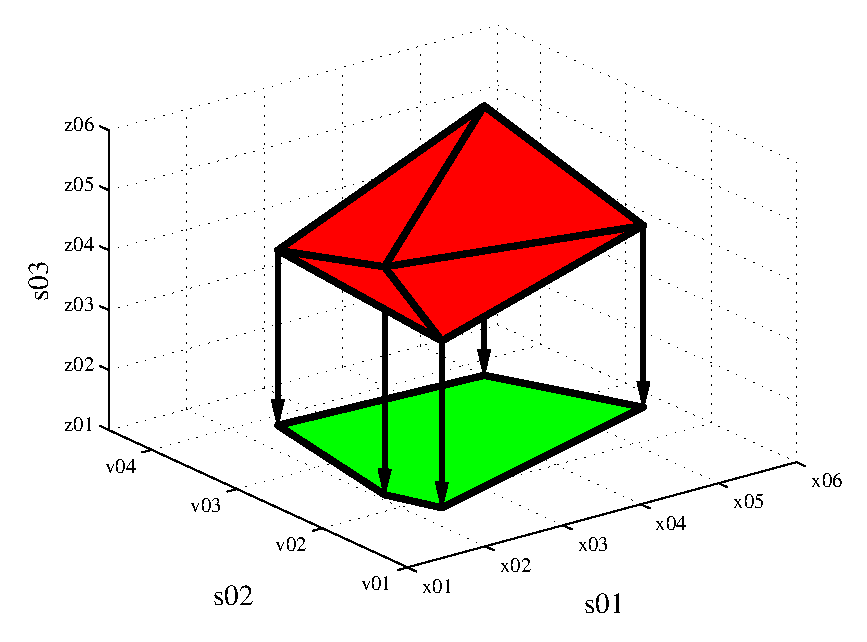
\includegraphics{fig_4_6_tex.eps}}%
\end{psfrags}%
%
% End fig_4_6_tex.tex
\end{document}
% See http://www.mathworks.de/matlabcentral/fileexchange/loadFile.do?objectId=4638
% for recent versions of laprint.m.
%
% created by:           LaPrint version 3.16 (13.9.2004)
% created on:           11-Jul-2009 20:16:30
% eps bounding box:     15 cm x 11.25 cm
% comment:              
%
\begin{psfrags}%
\psfragscanon%
%
% text strings:
\psfrag{s01}[lt][lt]{\color[rgb]{0,0,0}\setlength{\tabcolsep}{0pt}\begin{tabular}{l}x_1\end{tabular}}%
\psfrag{s02}[rt][rt]{\color[rgb]{0,0,0}\setlength{\tabcolsep}{0pt}\begin{tabular}{r}x_2\end{tabular}}%
\psfrag{s03}[b][b]{\color[rgb]{0,0,0}\setlength{\tabcolsep}{0pt}\begin{tabular}{c}x_3\end{tabular}}%
%
% xticklabels:
\psfrag{x01}[t][t]{-1}%
\psfrag{x02}[t][t]{-0.5}%
\psfrag{x03}[t][t]{0}%
\psfrag{x04}[t][t]{0.5}%
\psfrag{x05}[t][t]{1}%
\psfrag{x06}[t][t]{1.5}%
%
% yticklabels:
\psfrag{v01}[r][r]{-2}%
\psfrag{v02}[r][r]{-1}%
\psfrag{v03}[r][r]{0}%
\psfrag{v04}[r][r]{1}%
%
% zticklabels:
\psfrag{z01}[r][r]{0}%
\psfrag{z02}[r][r]{1}%
\psfrag{z03}[r][r]{2}%
\psfrag{z04}[r][r]{3}%
\psfrag{z05}[r][r]{4}%
\psfrag{z06}[r][r]{5}%
%
% Figure:
\resizebox{12cm}{!}{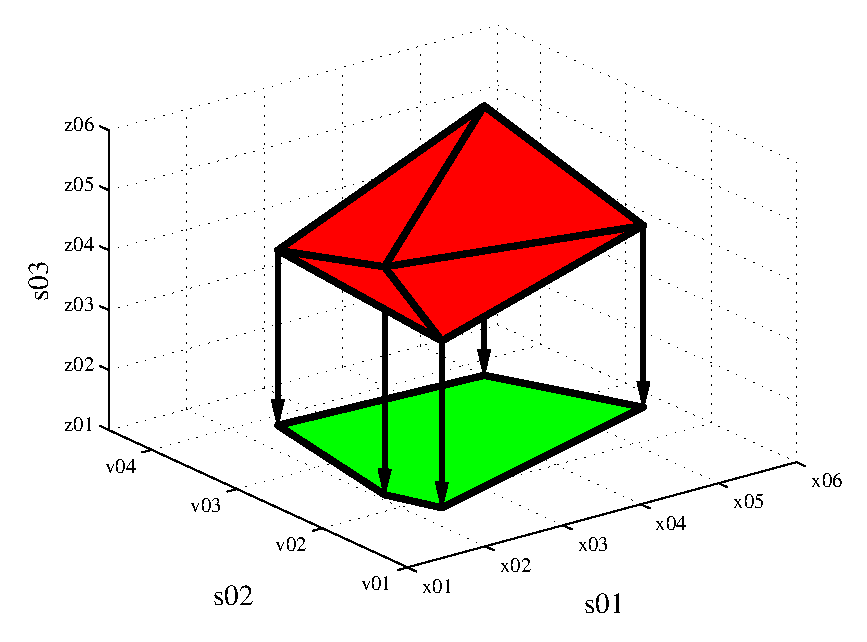
\includegraphics{fig_4_6_tex.eps}}%
\end{psfrags}%
%
% End fig_4_6_tex.tex
